\chapter{Overview}
This Chapter provides an overview of the problem, its motivation, and a general overview.

%%%%%%%%%%%%%%%%%%%%%%%%%%%%%%%%%%%%%%%%%%%%%%%%
\section{Literature Classification}
In this section, we explore some classifications related to AI safety-critical systems. This is useful for providing a general overview of the context of this work.

%%%%%%%%%%%%%
\subsection{Types of AI}
\label{sec:TAI}
In the literature, there are many types of AI (TAI). In this section, we provide a brief recap of them, as they may be useful in the following sections.
\begin{itemize}
    \item \textbf{Connectionists} \\
    These are models where training is performed using an optimization technique, most commonly gradient descent. Examples include Neural Networks (e.g., CNNs, Transformers).
    \item \textbf{Bayesian} \\
        These are models where results are obtained in a probabilistic manner.
    \item \textbf{Symbolists} \\
        These use logic to perform reasoning (e.g., decision trees and Prolog). Given that inference must validate all parts of the logic (i.e., each component of a Boolean expression) learned during the training phase, these models are useful if we want explainable models (e.g., in the \href{https://github.com/edoardosarri24/violation-prediction-in-realtime-system}{prediction of faults} in real-time scenarios).
    \item \textbf{Analogizers} \\
        These are usually classification models based on a similarity score (e.g., k-NN, SVM).
\end{itemize}

%%%%%%%%%%%%%
\subsection{Automation Levels}
When an AI-based system interacts with a human, the interaction can be done with different magnitudes. The EASA (European Union Aviation Safety Agency) defines three levels of automation and assistance~\cite{agirre2025functional}:
\begin{enumerate}
    \item EASA Level 1 \\
        This level refers to Collaborative Robots, which work side by side with humans without having total independence.
    \item EASA Level 2 \\
        The automatic systems operate in a closed environment. In this case, the system executes in a predefined environment where requirements are known during the design phase.
    \item EASA Level 3 \\
        The autonomous systems operate in an open environment. ISO 22989 defines this as the highest level of automation~\cite{perez2024artificial}, in which the system can modify its behavior and goals without human control.
\end{enumerate}

%%%%%%%%%%%%%
\subsection{Safety Standards}
\label{sec:standard}
Moving from traditional methods of guaranteeing safety to using AI to achieve it requires defining a new class of standards. The most common problem is related to the probability of failure: the most critical Safety Integrity Levels (SIL, ASIL, or DAL) require a very low probability of failure (e.g., $10^{-9}$), whereas excellent accuracy for an AI model is often 99\%. Thus, common AI models do not comply with these requirements.
\begin{itemize}
    \item \textbf{Traditional safety standards} \\
        Their objective is to mitigate risks using programmable functions, known as Safety Instrumented Systems (SIS), which are embedded in the system. The reliability of a SIS is defined by different measures depending on the domain: these include the Safety Integrity Level (SIL) for industry (IEC 61508), the Automotive Safety Integrity Level (ASIL) for the automotive sector (ISO 26262), and the Design Assurance Level (DAL) for aerospace (DO-178C).
    \item \textbf{AI Safety Standards} \\
        For heteronomous systems (e.g., Advanced Driver Assistance Systems (ADAS)), failures can occur even in the absence of hardware or software faults. This means that these new algorithms must comply with the Safety of the Intended Functionality (SOTIF) standard (ISO 21448), bringing them into alignment with classical FuSa.
\end{itemize}

%%%%%%%%%%%%%
\subsection{Points of Application}
\label{sec:application}
In this section, we recap the different types of AI applications. There are three categories that describe \textit{when} and \textit{how} an AI model can be used.
\begin{itemize}
    \item \textbf{Product} \\
        A safety-critical system relies on one or more safety functions based on an AI model. This model is offline: training is performed before the model is embedded in the system.
    \item \textbf{Runtime} \\
        This is similar to the previous category, but the model can update itself during execution.
    \item \textbf{Process} \\
        The system itself does not include an AI model, but it is designed and developed using AI models (e.g., generative AI to generate code or run tests).
\end{itemize}

\myskip

Based on this classification, ISO 5469 defines three classes for when AI models can be included in a safety-critical system (i.e., product, runtime, and process) while complying with the standards defined in Section~\ref{sec:standard}.
\begin{itemize}
    \item \textbf{Class I} \\
        These systems are based on traditional AI models, such as those referred to as \textit{symbolists} in Section~\ref{sec:TAI}. Since they are totally deterministic and formal verification can be performed, these models comply with classic FuSa.
    \item \textbf{Class II} \\
        The system contains an AI model that may not be compliant with FuSa on its own. Compliance is achieved through a runtime checker, often known as a \textit{safety bag}; if the model fails, the checker detects the failure and makes a safe choice.
    \item \textbf{Class III} \\
        These are systems that cannot incorporate an AI model internally. In this case, the solution is usually to include the model, but engineers do not take responsibility for possible failures (e.g., ADAS in vehicles).
\end{itemize}

%%%%%%%%%%%%%%%%%%%%%%%%%%%%%%%%%%%%%%%%%%%%%%%%
\section{AI-Based Safety-Critical Systems}
Although integrating AI into a safety-critical system can be very challenging, there are many techniques that can be used and have already been tested. For example, referring to the classification in Section~\ref{sec:application}, we find that \textit{Class I} and \textit{Class II} include systems that are already on the market (e.g., SIL4 railway interlockings).

Usually, these systems are composed of the elements shown in Figure~\ref{fig:AI_system}: the entire system consists of an AI system, which is defined by an execution platform and the AI item.
\begin{figure}[htbp]
    \centering
    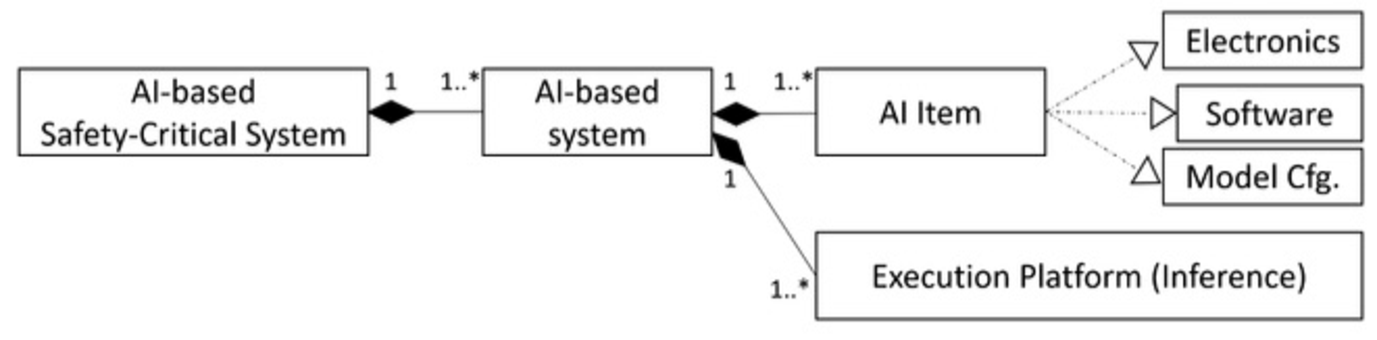
\includegraphics[max width=\textwidth, max height=0.85\textheight, keepaspectratio]{images/2-overview/AI_system_components.pdf}
    \caption{AI-Based safety-critical system components~\cite{perez2024artificial}.}
    \label{fig:AI_system}
\end{figure}

%%%%%%%%%%%%%
\subsection{Product}
As mentioned in Section~\ref{sec:application}, the product class describes a safety-critical system that relies for its SIS on one or more AI-based functions trained offline. These functions can be ``simple'', as in the case of a symbolist AI model, thus belonging to \textit{Class I}, or they can be very complex and belong to \textit{Class II}. In the first case, since the model is deterministic, we can use formal verification to ensure the system's compliance with FuSa. In the second case, the standard industry technique is to use a runtime checker that makes a safe choice for the next action if the model operates outside its requirements or produces an unsafe result.

\subsubsection{Testing}
The main problem with these AI-based safety-critical systems is the safety assurance we can assign to them. This derives from the stochastic nature of AI models, which implies that they can have \textit{uncertainty-induced failures}; to reduce this uncertainty, we must investigate unknown factors. Therefore, when describing safety functions in this scenario, we speak about the intended functionality: their design is a set of high-level objectives rather than a set of precise and well-defined instructions. This can be mitigated by applying formal verification methods, but even in this case, the black-box nature of the models suggests that these methods cannot be the only ones. Another challenge is testing the AI model itself, which is a widely explored area (e.g., test generation using an NLP model).

\subsubsection{Neural Networks}
Although symbolist models provide understandability and explainability of their decisions, the most powerful models are Neural Networks (NNs).

When dealing with these kinds of models, we must consider several detailed issues:
\begin{itemize}
    \item Supervised learning relies on data. When managing data (i.e., preprocessing and dividing data into training and test sets), we must do so with high precision.
    \item This is an area where \textit{changing nothing changes everything}~\cite{perez2024artificial}. This means that changing activation functions and hyperparameters can lead to very different behaviors.
    \item NN training is iterative; this must be included in the V-Model during the specification and testing phases.
    \item AI frameworks (e.g., PyTorch) are general-purpose and user-friendly. However, there are some APIs that also provide a set of safety requirements.
\end{itemize}

%%%%%%%%%%%%%
\subsection{Runtime}
\label{sec:runtime}
As discussed in Section~\ref{sec:application}, a runtime safety-critical system is able to manage its AI module during execution. These are notable systems because they allow the SIS to evolve with the context: a case study reported a gas turbine where the safety function evolves as the engine degrades.

This kind of solution bases its dependability and standard compliance on five different techniques:
\begin{itemize}
    \item \textbf{Safety Bag} \\
        This is the same technique mentioned above: a runtime checker monitors the AI model's results, and if it detects anomalous behavior, it produces a safe output.
    \item \textbf{Safe Adaptation} \\
        Both the AI model and the (continuous) training algorithm conform to safety standards.
    \item \textbf{Limited Adaptation} \\
        The (continuous) training is limited within a safe range: this means that even if the weights of the model change, they cannot do so by a large magnitude.
    \item \textbf{Limited Actuation} \\
        In this case, the adaptation is performed with hard constraints on the resulting model's output: for example, the new model cannot produce an output whose magnitude exceeds a certain threshold.
    \item \textbf{Library-Based Offline} \\
        We train a set of AI models, each of which conforms to safety standards. During inference, the system chooses among the available models in a non-linear way (i.e., with \texttt{if/else}).
\end{itemize}

%%%%%%%%%%%%%
\subsection{Process}
These are offline solutions that support engineers in designing safety-critical systems, both for the overall system and the AI component that implements the safety function.

\myskip

In traditional safety engineering, AI models can be useful for validating and assessing the V-Model. During specification, we can use an NLP model (e.g., Transformer-based) to discover hazards and issues in the process; during design and implementation, models can be useful for generating code; and during the testing phase, they are useful for generating test cases.

If we look at the use of AI to construct other models that will implement safety functions, there are different solutions: in AutoML, we use reinforcement learning to find the best model hyperparameters, and we can implement models that search exhaustively for all combinations to test our system.